
\begin{frame}{The Problem}

  \begin{center}
    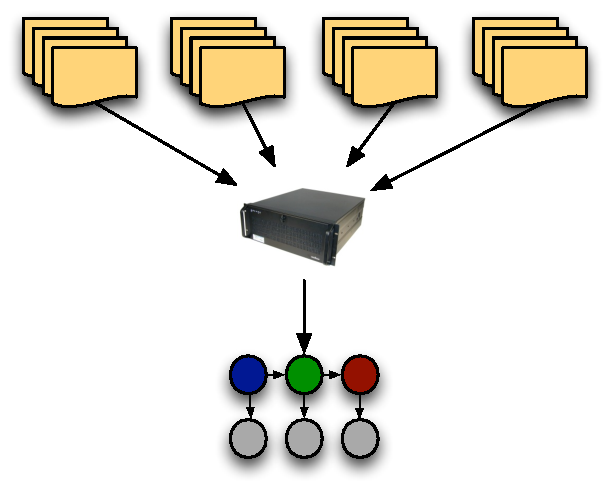
\includegraphics[width=.7\linewidth]{infvoc/batch} \\
    Batch algorithms can't scale
  \end{center}

\end{frame}

\begin{frame}{One Solution: Parallelization}
  \begin{center}
    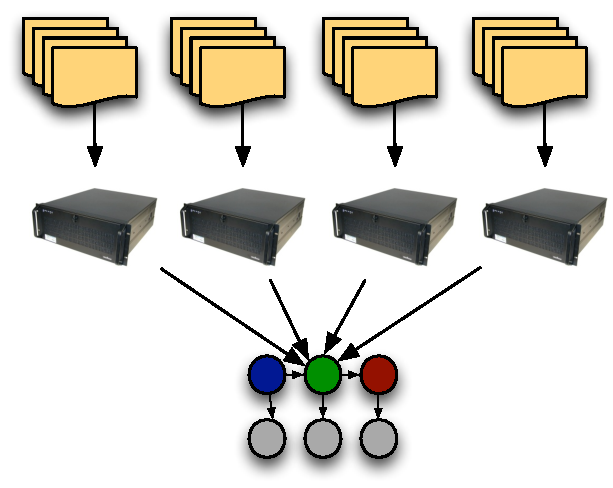
\includegraphics[width=.7\linewidth]{infvoc/parallel} \\
    Throw more computers at the problem \\
    For topic models, \textsc{Mr Lda}~\cite{zhai-12}
  \end{center}
\end{frame}

\begin{frame}{Another Solution: Streaming Algorithms}
  \begin{center}
    \only<1>{ 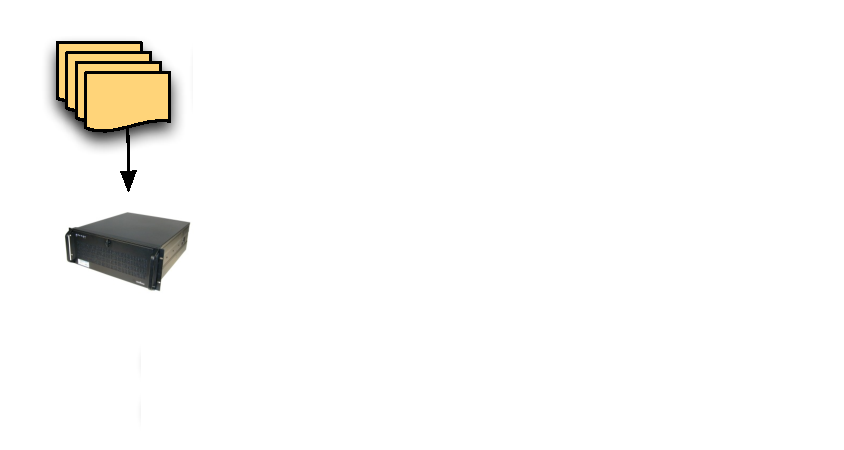
\includegraphics[width=.8\linewidth]{infvoc/streaming-0}}
    \only<2>{ 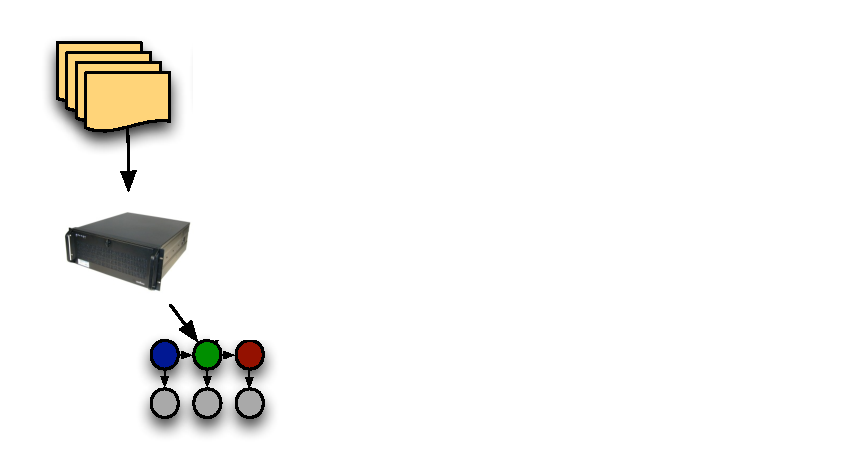
\includegraphics[width=.8\linewidth]{infvoc/streaming-1}}
    \only<3>{ 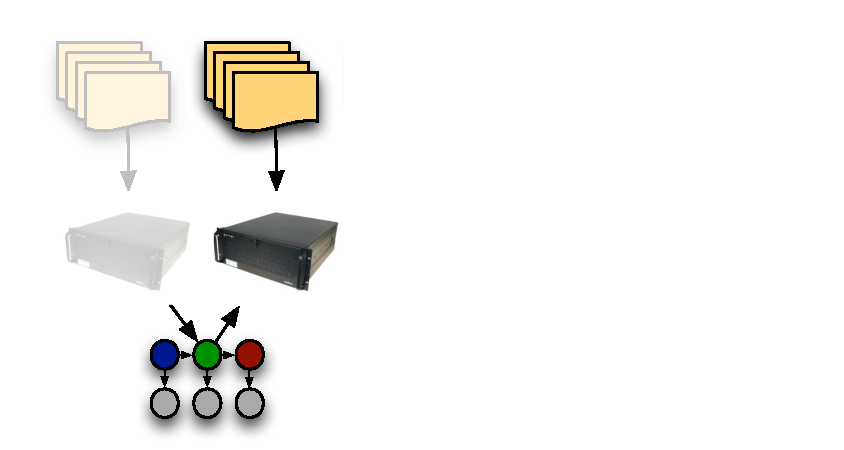
\includegraphics[width=.8\linewidth]{infvoc/streaming-2}}
    \only<4>{ 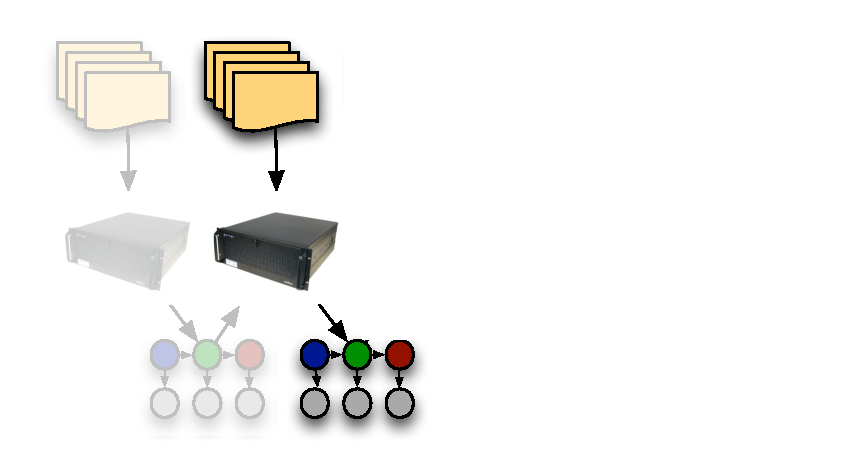
\includegraphics[width=.8\linewidth]{infvoc/streaming-3}}
    \only<5>{ 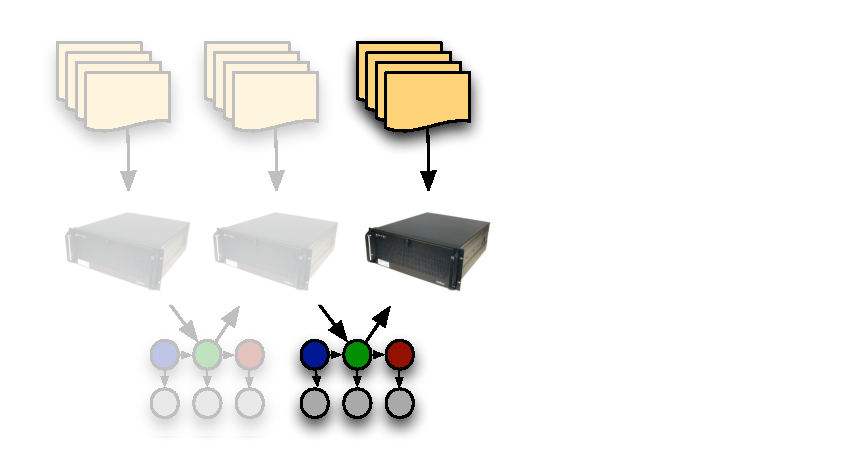
\includegraphics[width=.8\linewidth]{infvoc/streaming-4}}
    \only<6>{ 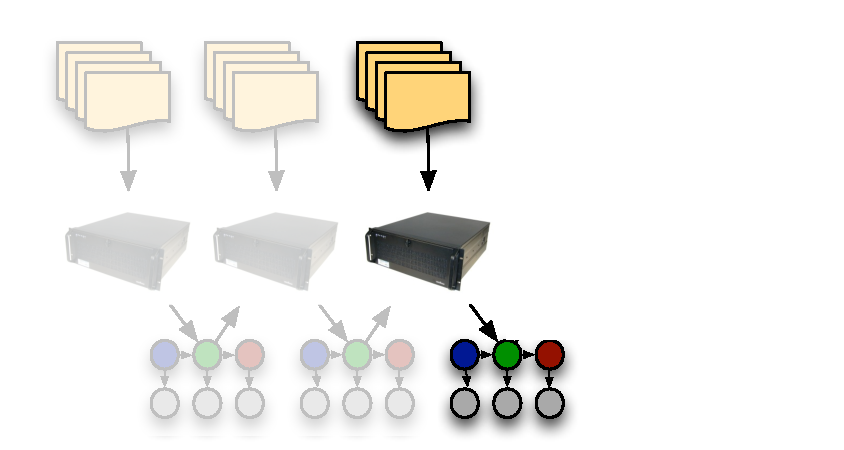
\includegraphics[width=.8\linewidth]{infvoc/streaming-5}}
    \only<7>{ 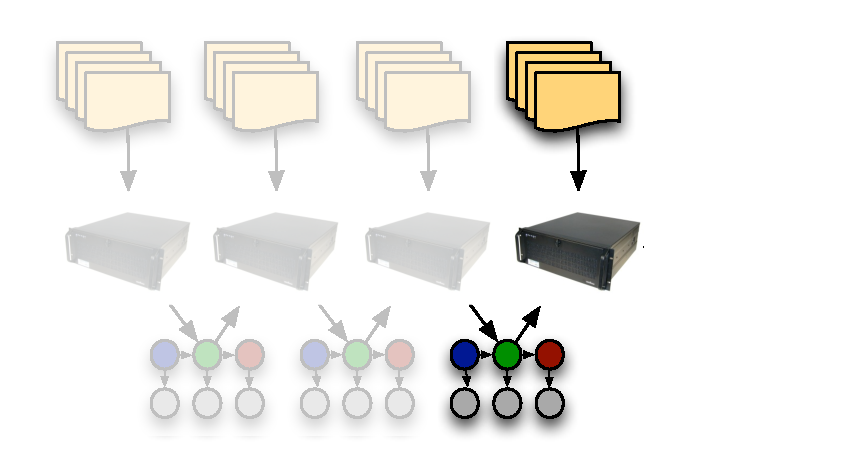
\includegraphics[width=.8\linewidth]{infvoc/streaming-6}}
    \only<8>{ 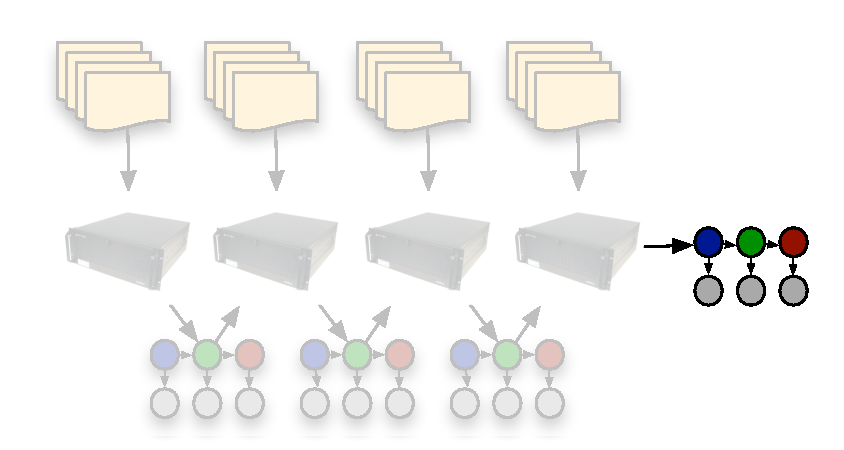
\includegraphics[width=.8\linewidth]{infvoc/streaming-7}}
    \\
    Handle the data as they come
  \end{center}
\end{frame}


% Making inference more efficient

% Streaming algorithms

% Why this is a problem for LDA

\begin{frame}{Streaming Topic Models}
\begin{itemize}
  \item There are streaming algorithms for topic models
    \begin{itemize}
       \item Gibbs sampling~\cite{yao-09}
       \item Variational inference~\cite{hoffman-10}
       \item Hybrid~\cite{mimno-12}
    \end{itemize}
  \item Retain batch traditional topic model's probabilistic model
\end{itemize}
\end{frame}


\begin{frame}{Finite Distributions}

  \begin{columns}
     \column{.5\linewidth}
     \centering
      $\phi_k \sim \mbox{Dir}(\alpha)$

   \begin{block}{Limitation}
     Finite fixed support, so you need to specify vocabulary up front.
\end{block}

     \column{.5\linewidth}
     \centering
       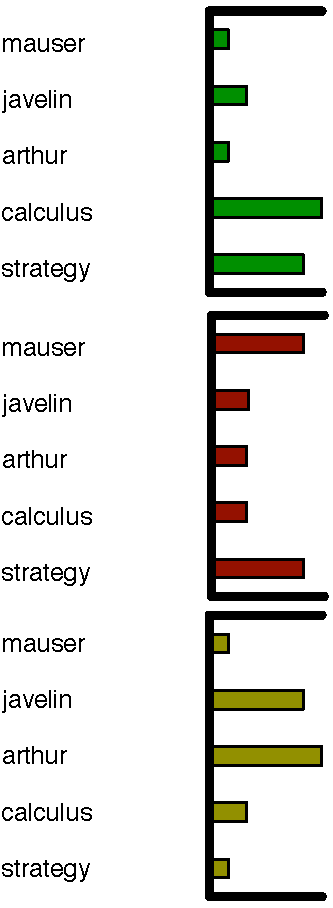
\includegraphics[width=.5\linewidth]{infvoc/finite_dirichlet}
  \end{columns}

\end{frame}

\begin{frame}{Streaming topic model's Problem}
\begin{itemize}
  \item It assumes a fixed vocabulary
  \item But new words constantly appear
    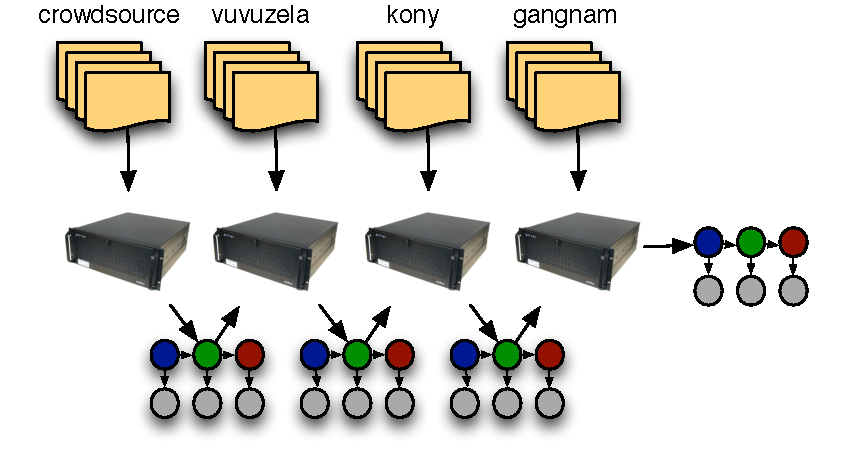
\includegraphics[width=.8\linewidth]{infvoc/streaming-words}
  \item You could miss out: leaders, memes
\pause
  \item Our solution: infinite vocabulary topic models
\end{itemize}
\end{frame}

% Nonparametric models

\begin{frame}{The Infinite Dirichlet Process}
  \only<1>{ 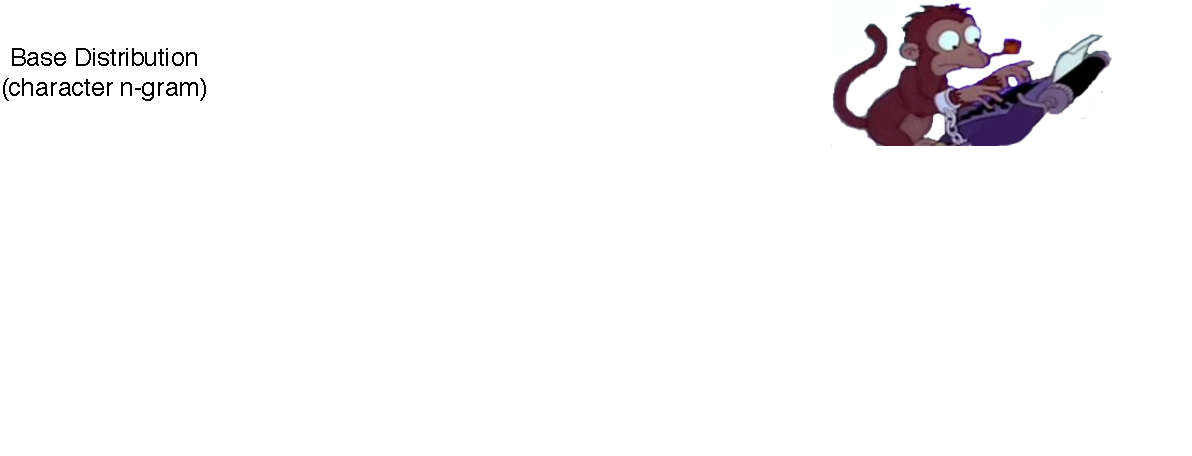
\includegraphics[width=.95\linewidth]{infvoc/dp_monkey-1} }
  \only<2>{ 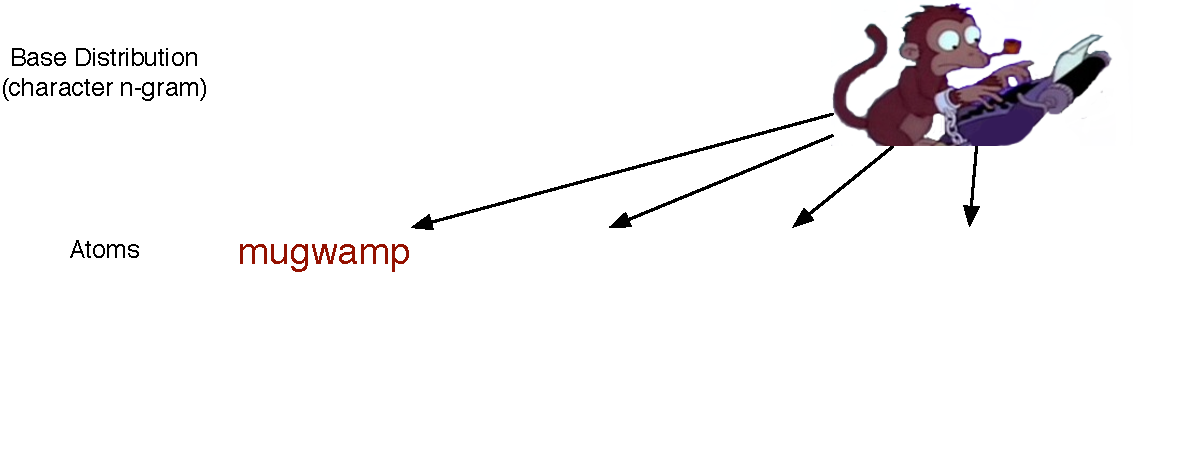
\includegraphics[width=.95\linewidth]{infvoc/dp_monkey-2} }
  \only<3>{ 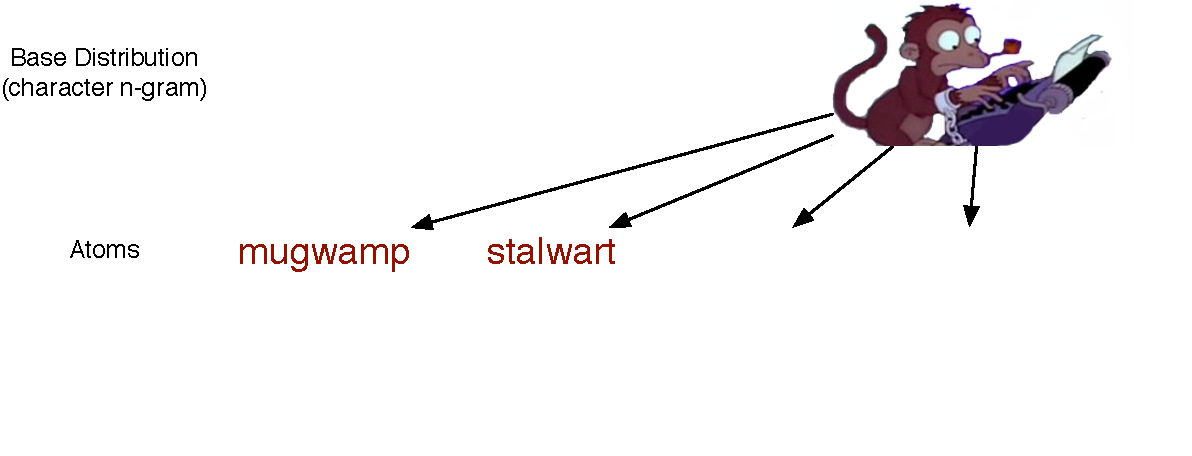
\includegraphics[width=.95\linewidth]{infvoc/dp_monkey-3} }
  \only<4>{ 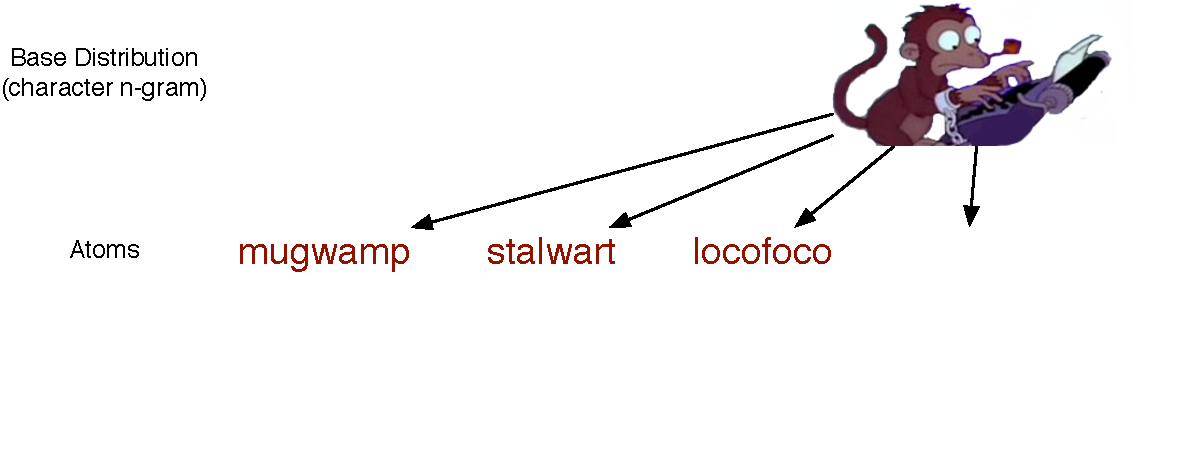
\includegraphics[width=.95\linewidth]{infvoc/dp_monkey-5} }
  \only<5>{ 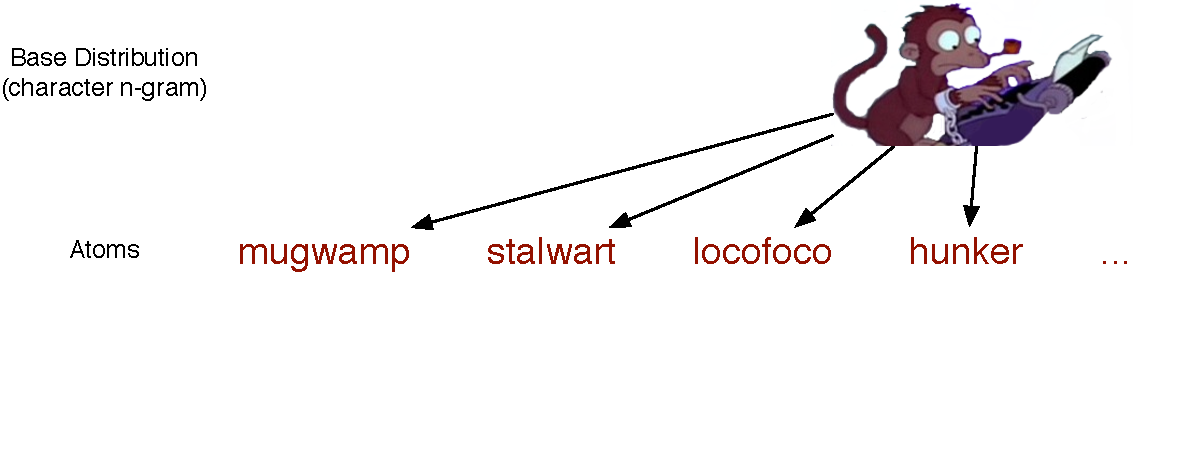
\includegraphics[width=.95\linewidth]{infvoc/dp_monkey-6} }
  \only<6>{ 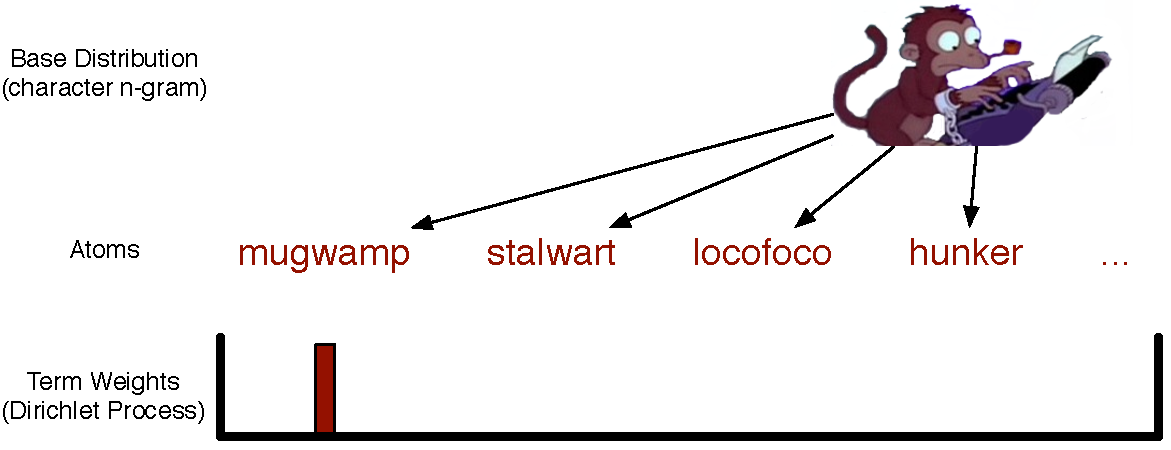
\includegraphics[width=.95\linewidth]{infvoc/dp_monkey-7} }
  \only<7>{ 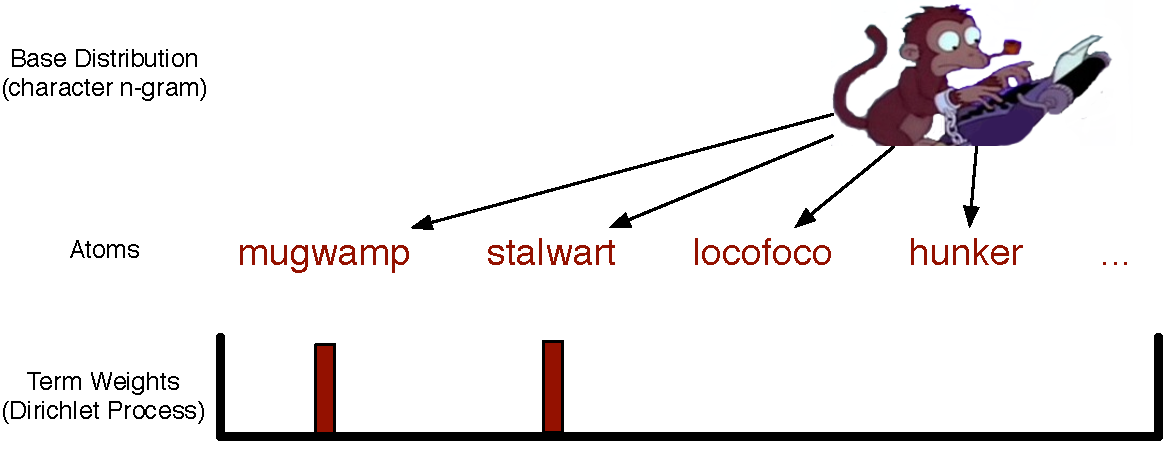
\includegraphics[width=.95\linewidth]{infvoc/dp_monkey-8} }
  \only<8>{ 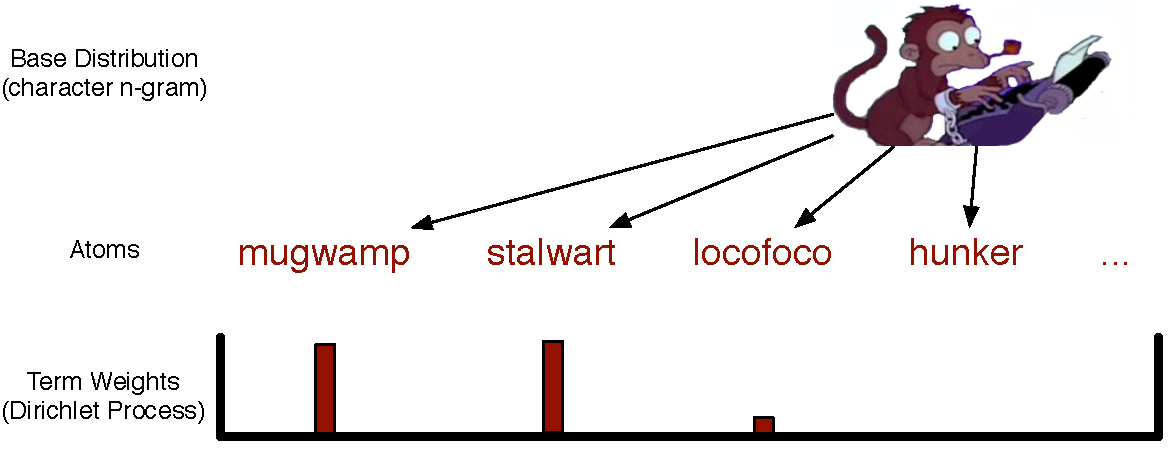
\includegraphics[width=.95\linewidth]{infvoc/dp_monkey-9} }
  \only<9>{ 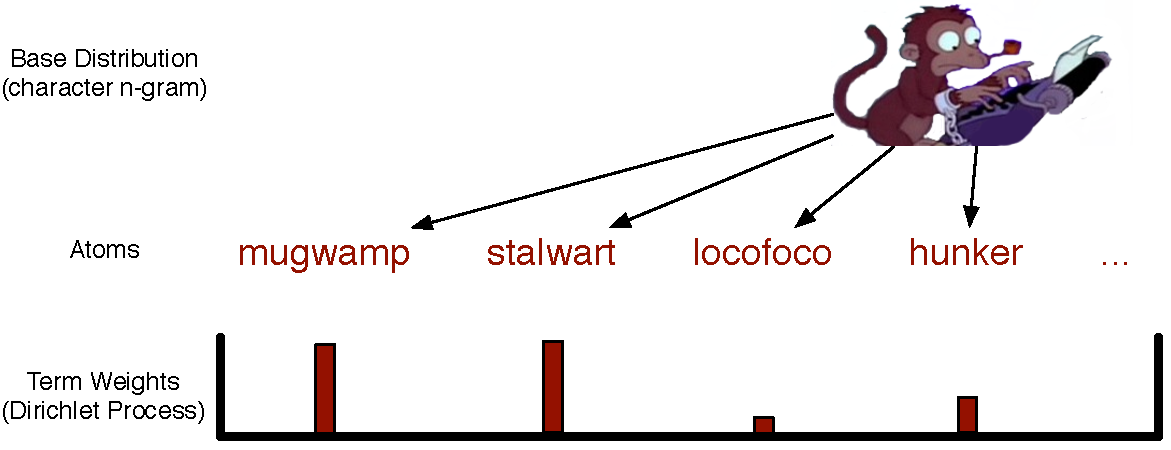
\includegraphics[width=.95\linewidth]{infvoc/dp_monkey-10} }
  \only<10->{ 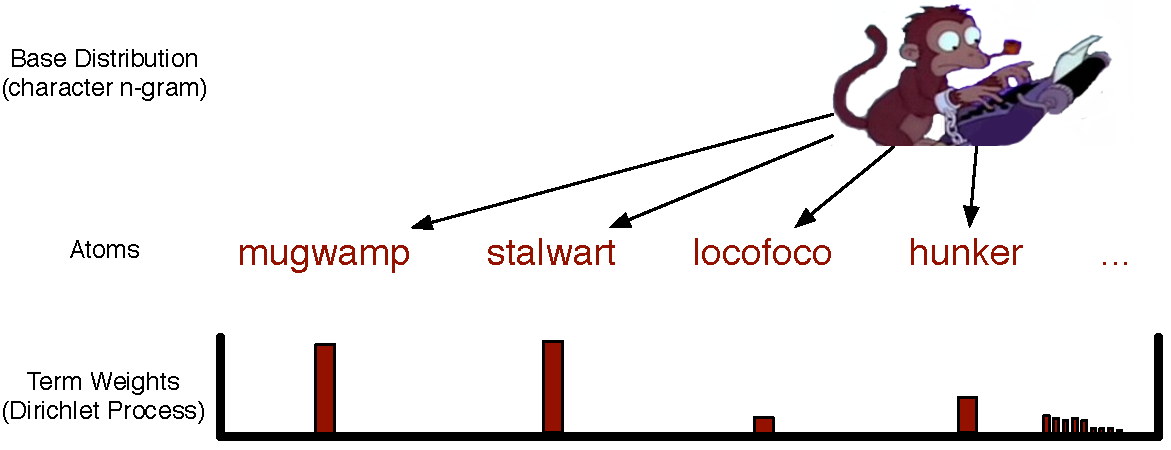
\includegraphics[width=.95\linewidth]{infvoc/dp_monkey-11} \\}
  \only<11->{Example of Bayesian nonparametrics \cite{ferguson-73,sethuraman-94}}
\end{frame}

% Our model

\begin{frame}{Infinite Vocabulary Topic Model}

  \begin{columns}
     \column{.44\linewidth}
     \begin{itemize}
       \item Each topic $\theta_k \sim \mbox{DP}(\alpha, G_0)$
       \item Infinite collection of atoms and weights
     \begin{itemize}
       \item For each word, ``stick breaks'' \alert<2>{$b_{k, w} \sim \mbox{Beta}(1,\alpha)$}
       \item Each atom gets weight \alert<3>{$\beta_{k, w} = \prod_{j=1}^{w} (1 - b_j)$}
       \item Atom identity drawn from base distribution $\rho_k \sim G_0$
     \end{itemize}
     \end{itemize}
     \column{.55\linewidth}
       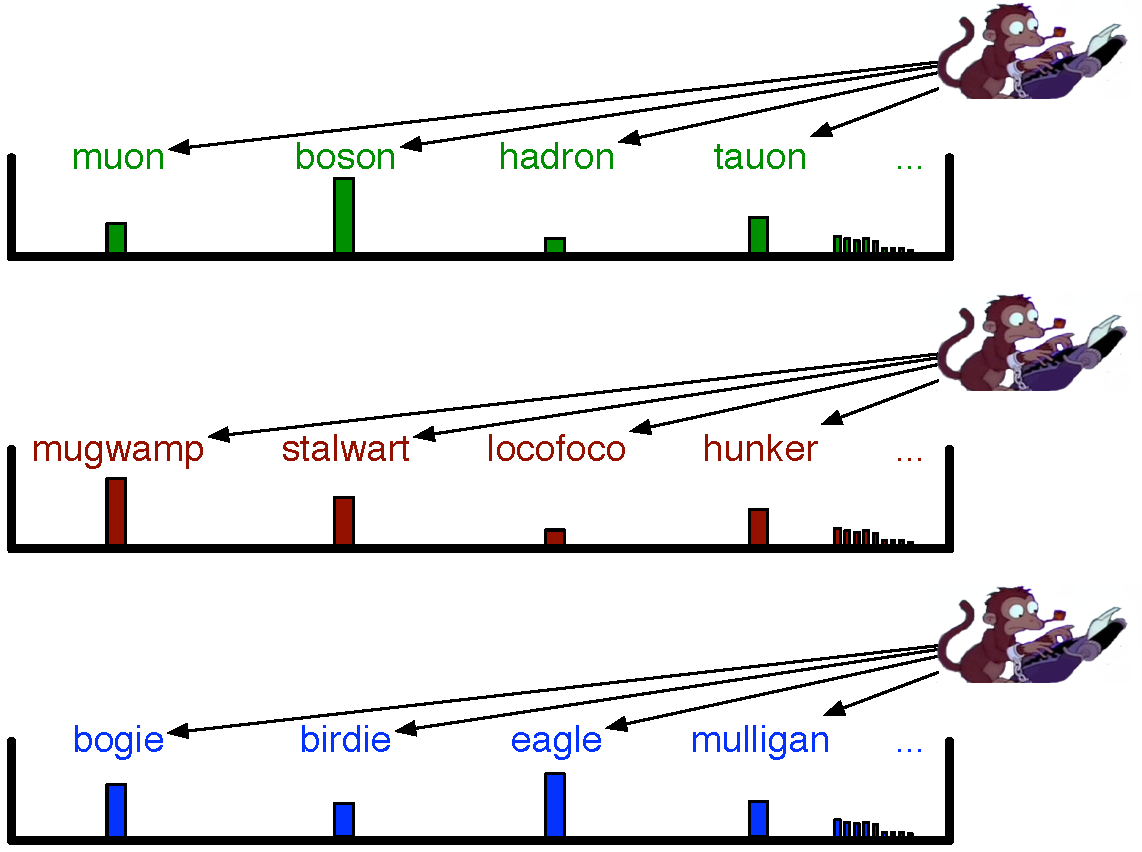
\includegraphics[width=1.0\linewidth]{infvoc/dp_monkey-topics}
  \end{columns}

\end{frame}

% Comics

\begin{frame}{Inference}

We can't optimize the joint likelihood
\begin{align}
& \textstyle p( \boldsymbol{W}, \boldsymbol{\rho}, \boldsymbol{\beta},
\boldsymbol{\theta}, \boldsymbol{z} ) = \prod_{k=1}^K
\left[ \prod_{t=1}^{\infty} p( \rho_{kt} | G_0 ) \cdot p( \beta_{kt}
| \alpha^{\beta} ) \right] \notag \\
& \textstyle \left[ \prod_{d=1}^{D} p( \boldsymbol{\theta}_d | \alpha^{\theta} )
\prod_{n=1}^{N_d} p( z_{dn} | \boldsymbol{\theta}_d ) p( \omega_{dn} |
z_{dn}, \boldsymbol{\beta}_{z_{dn}} ) \right] . \notag
\end{align}
\pause
so we optimize a lower bound of the objective based on a variational distribution $q$,
\begin{align}
\textstyle \log p(\boldsymbol{W}) \geq {\e{q(\boldsymbol{Z})}{\log p(\boldsymbol{W},\boldsymbol{Z})} - \e{q(\boldsymbol{Z})}{q}} = \elbo,
\label{eq:elbo-vague}
\end{align}
which we optimize $\elbo(\boldsymbol{Z})$ using gradient steps.
\end{frame}


\begin{frame}{Incorporating New Words}

\centering
       \only<1>{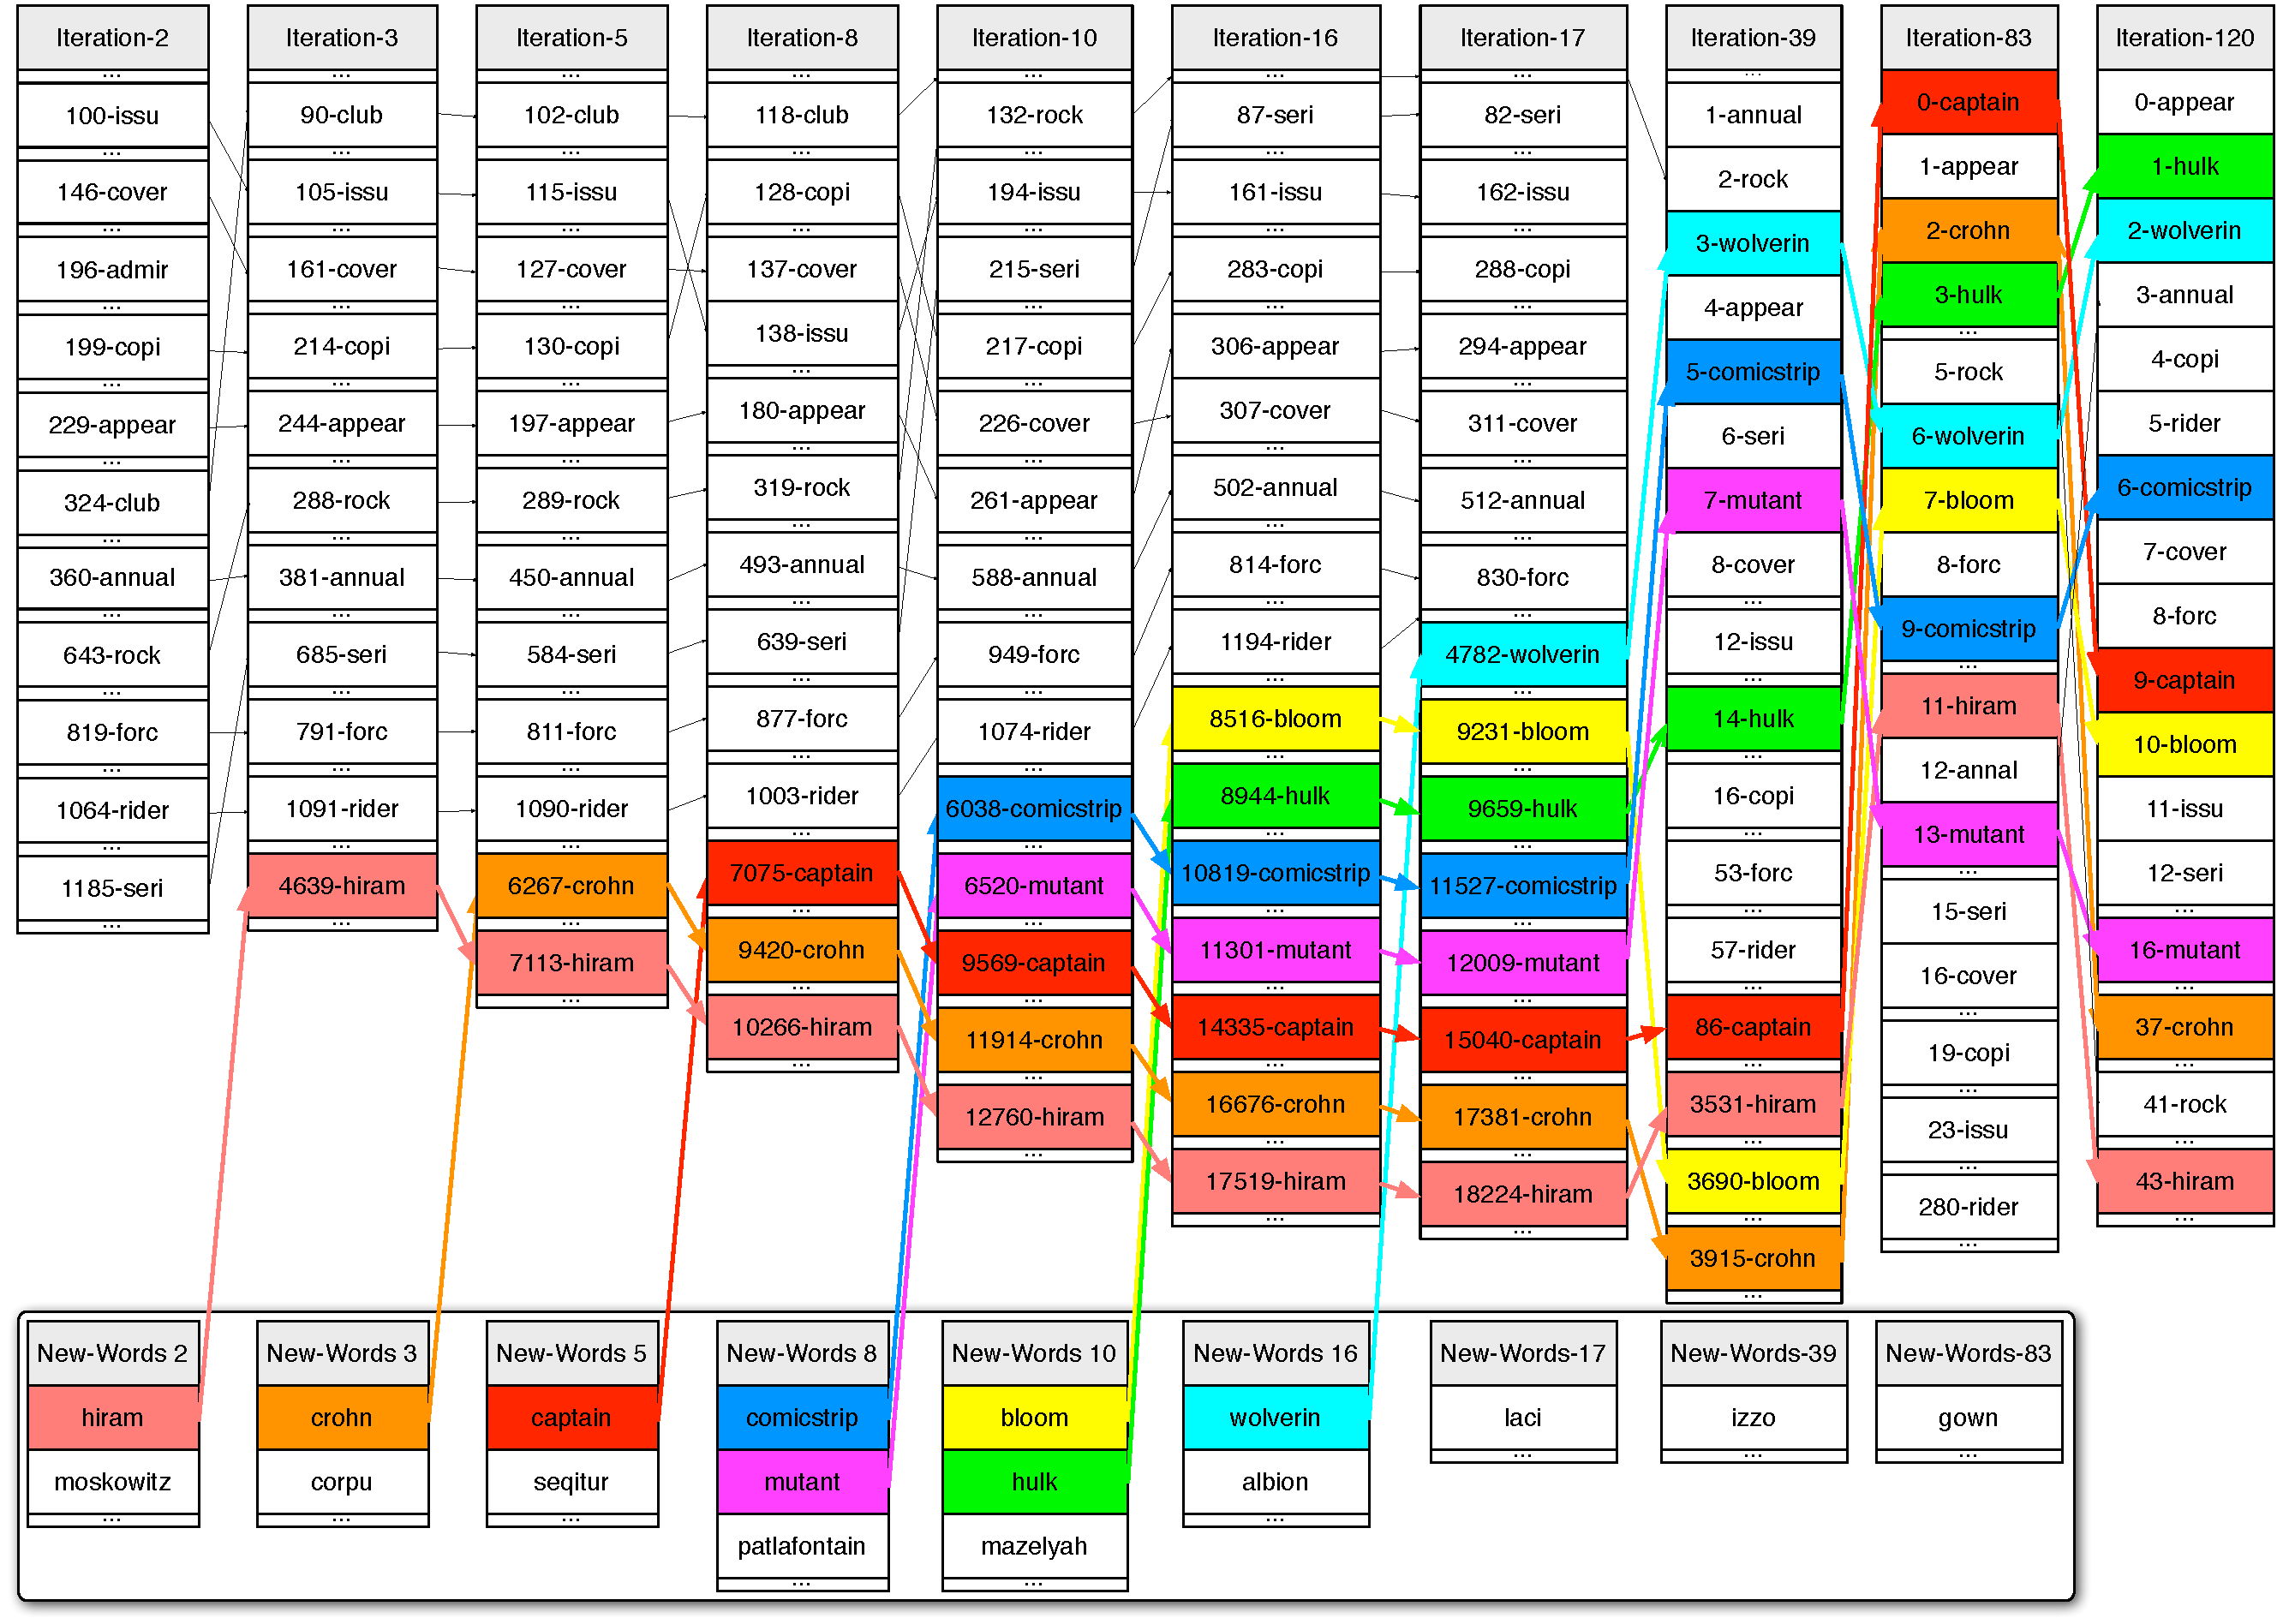
\includegraphics[width=1.0\linewidth]{infvoc/new_words_topic}}
       \only<2>{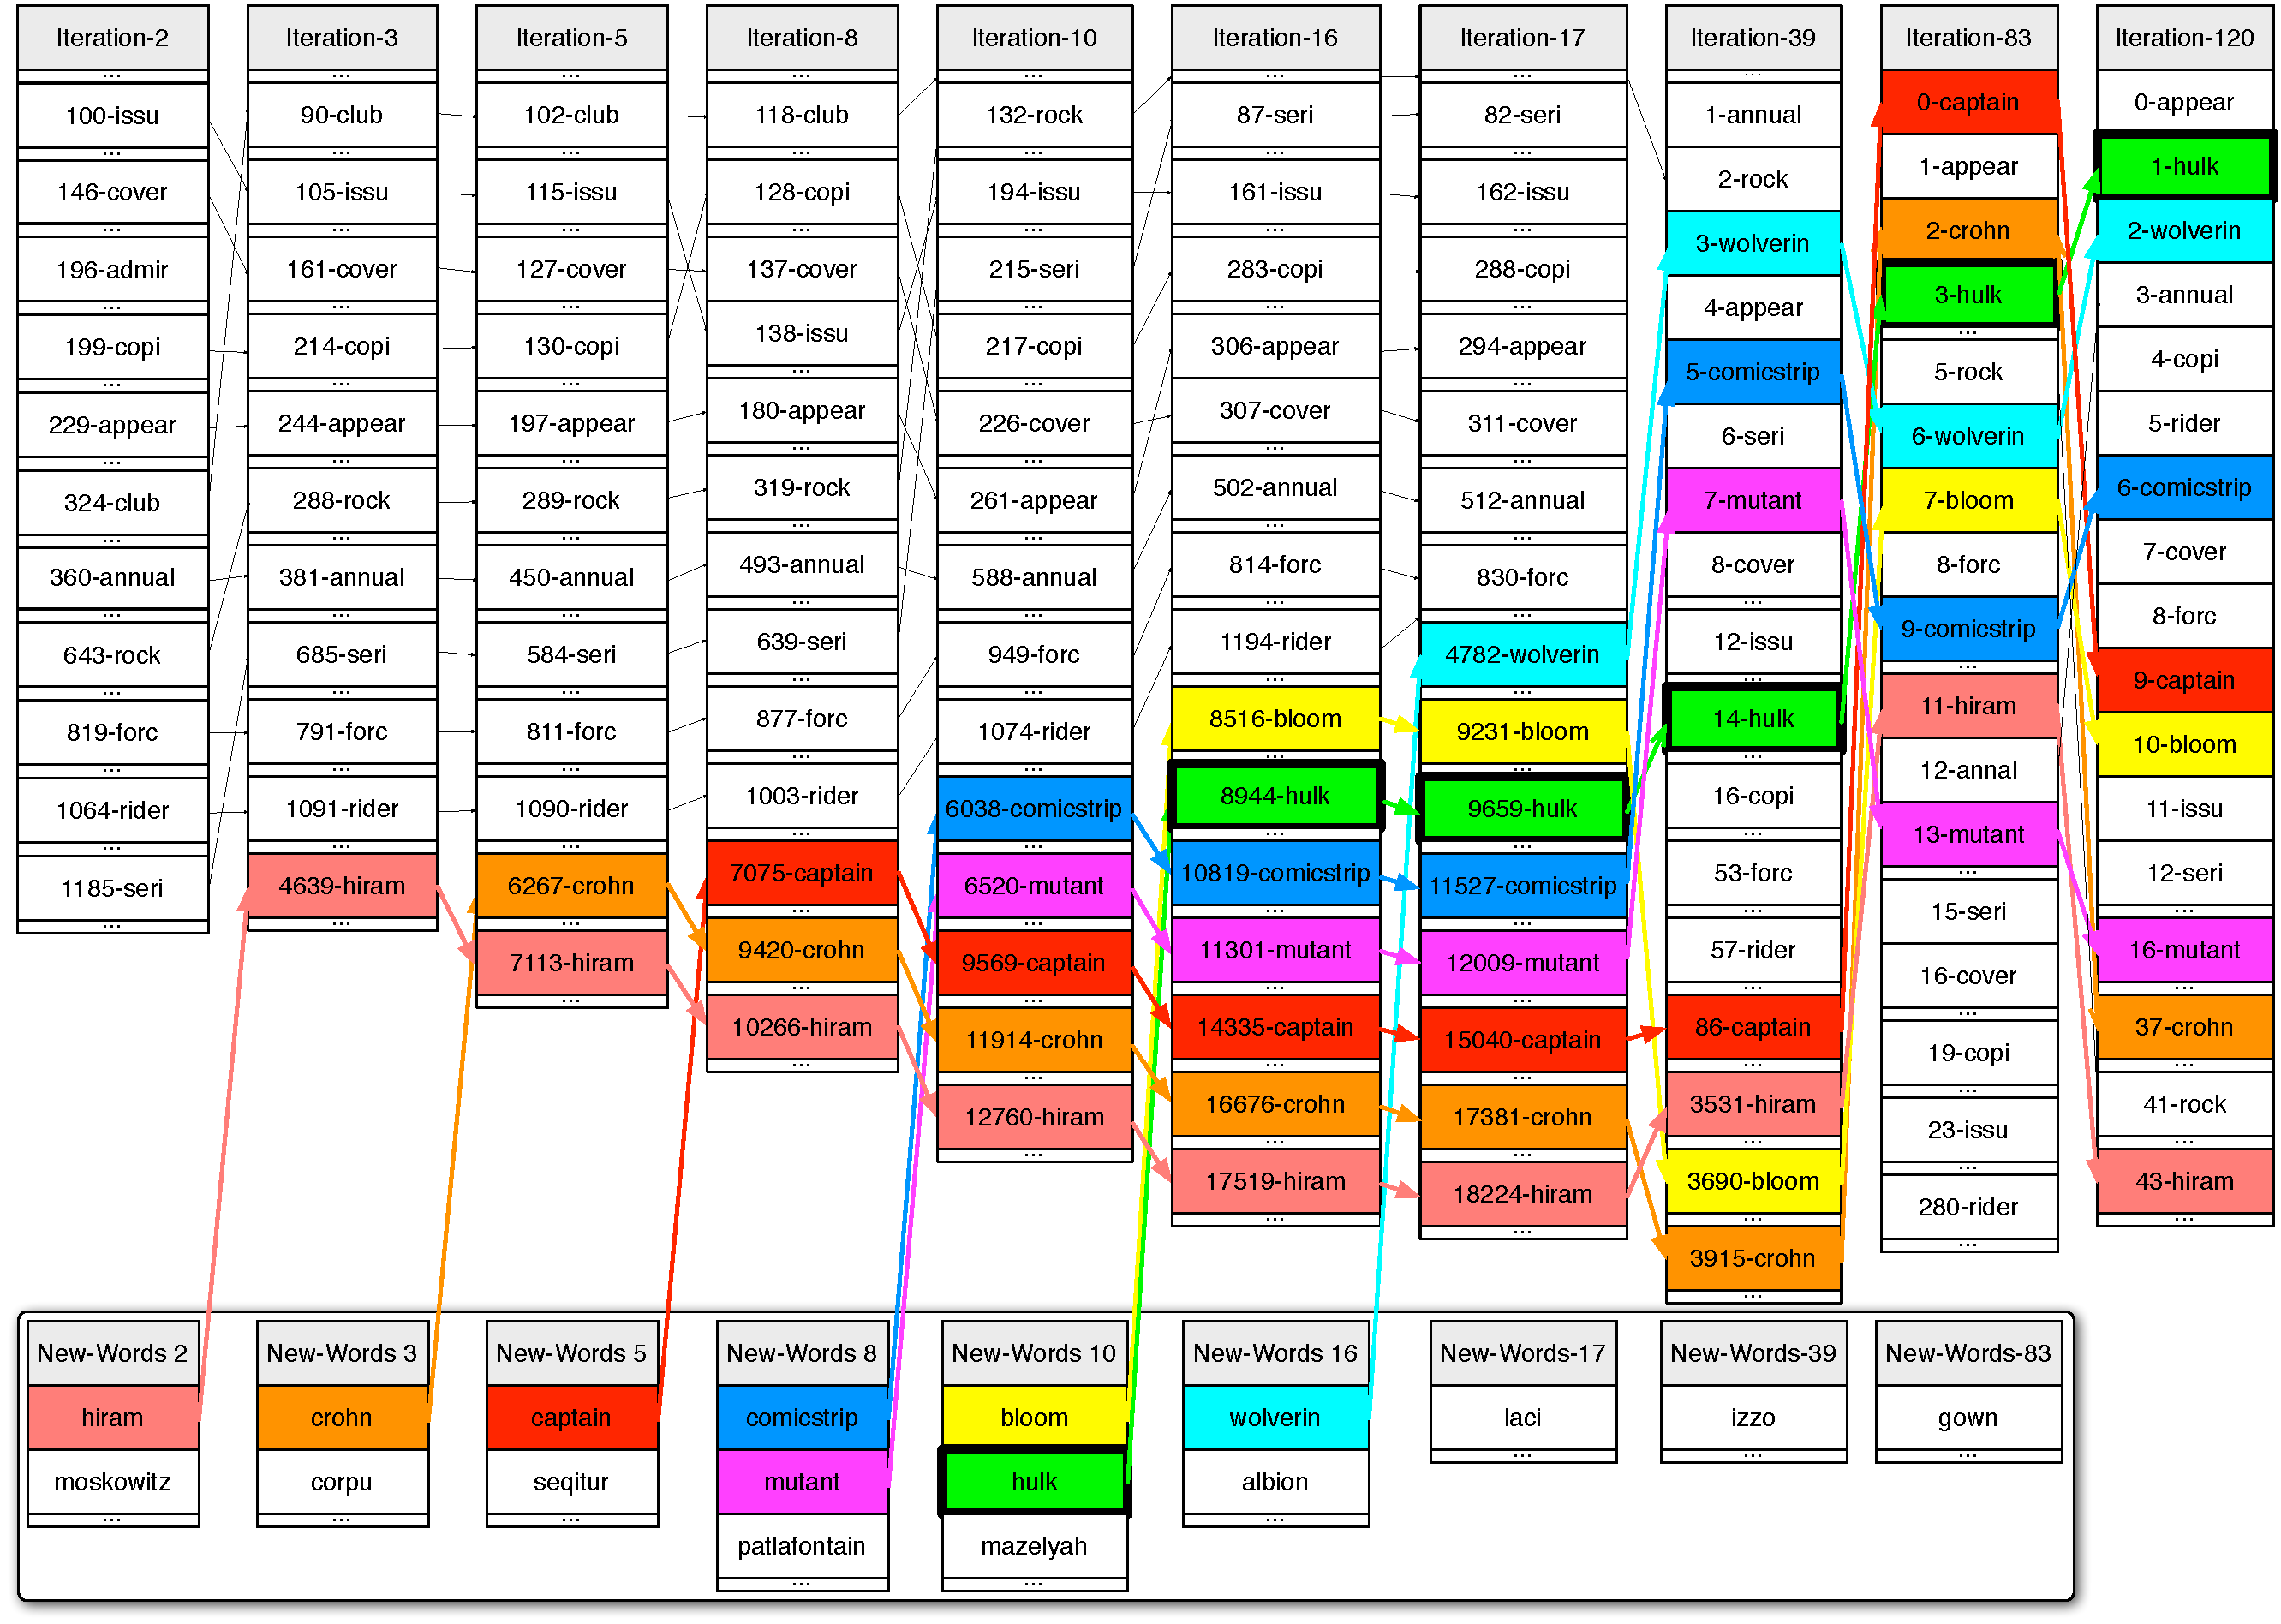
\includegraphics[width=1.0\linewidth]{infvoc/new_words_hulk}}
\end{frame}

\begin{frame}{Do the topics make sense?}

\centering
       \only<1>{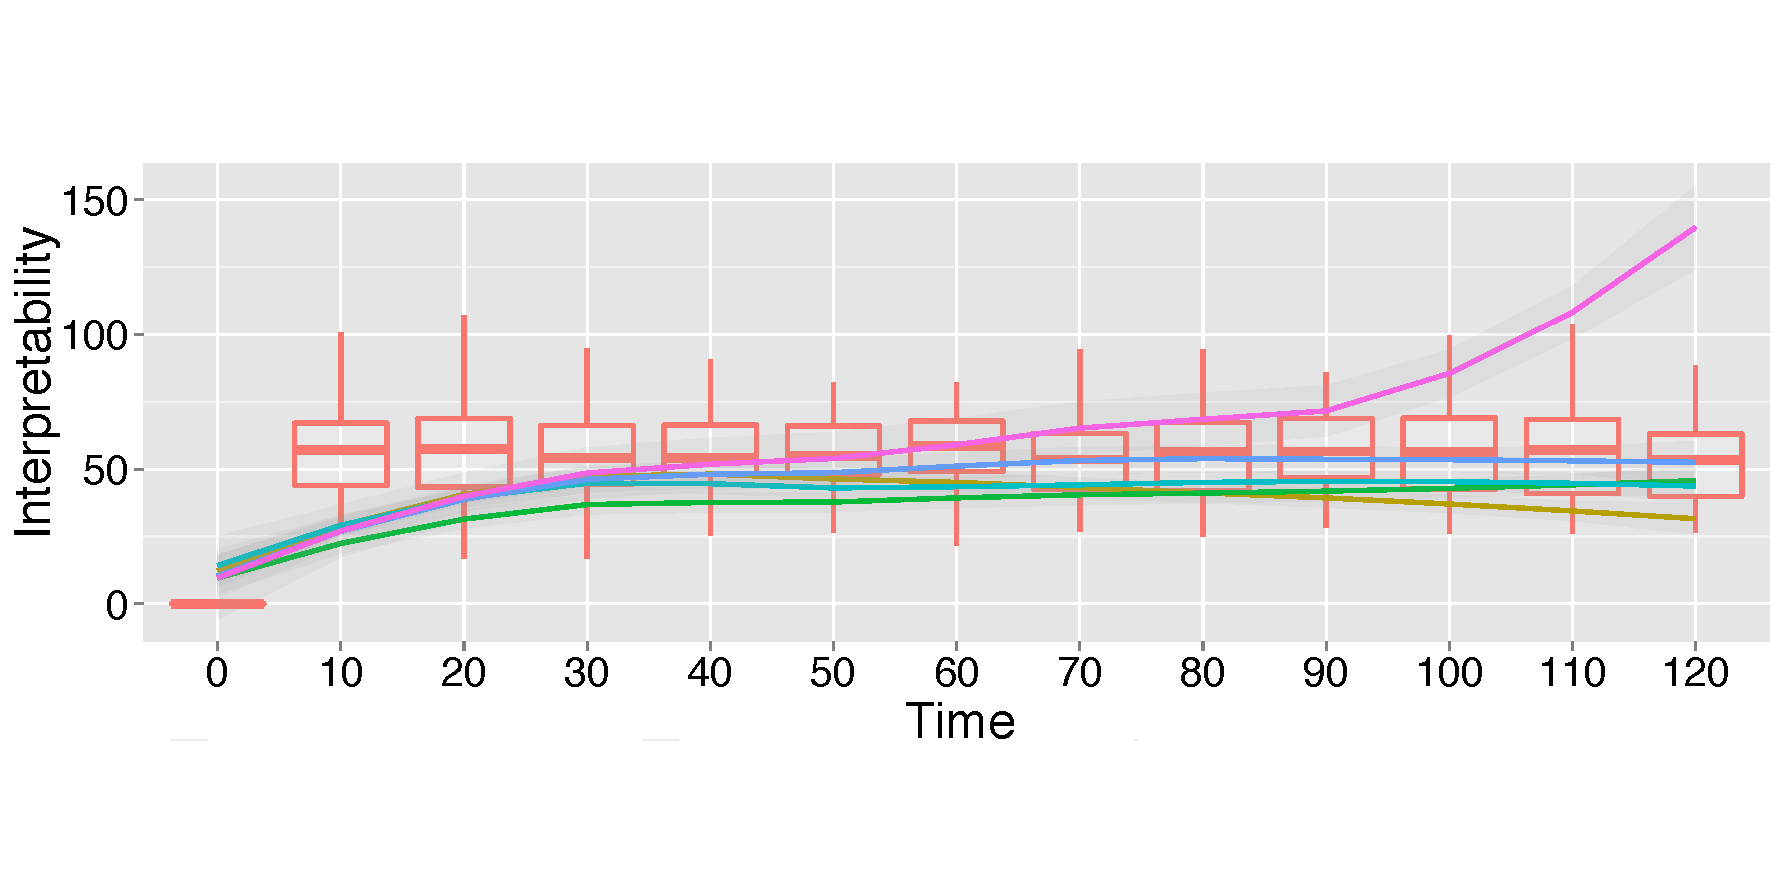
\includegraphics[width=1.0\linewidth]{infvoc/coherence_0}}
       \only<2>{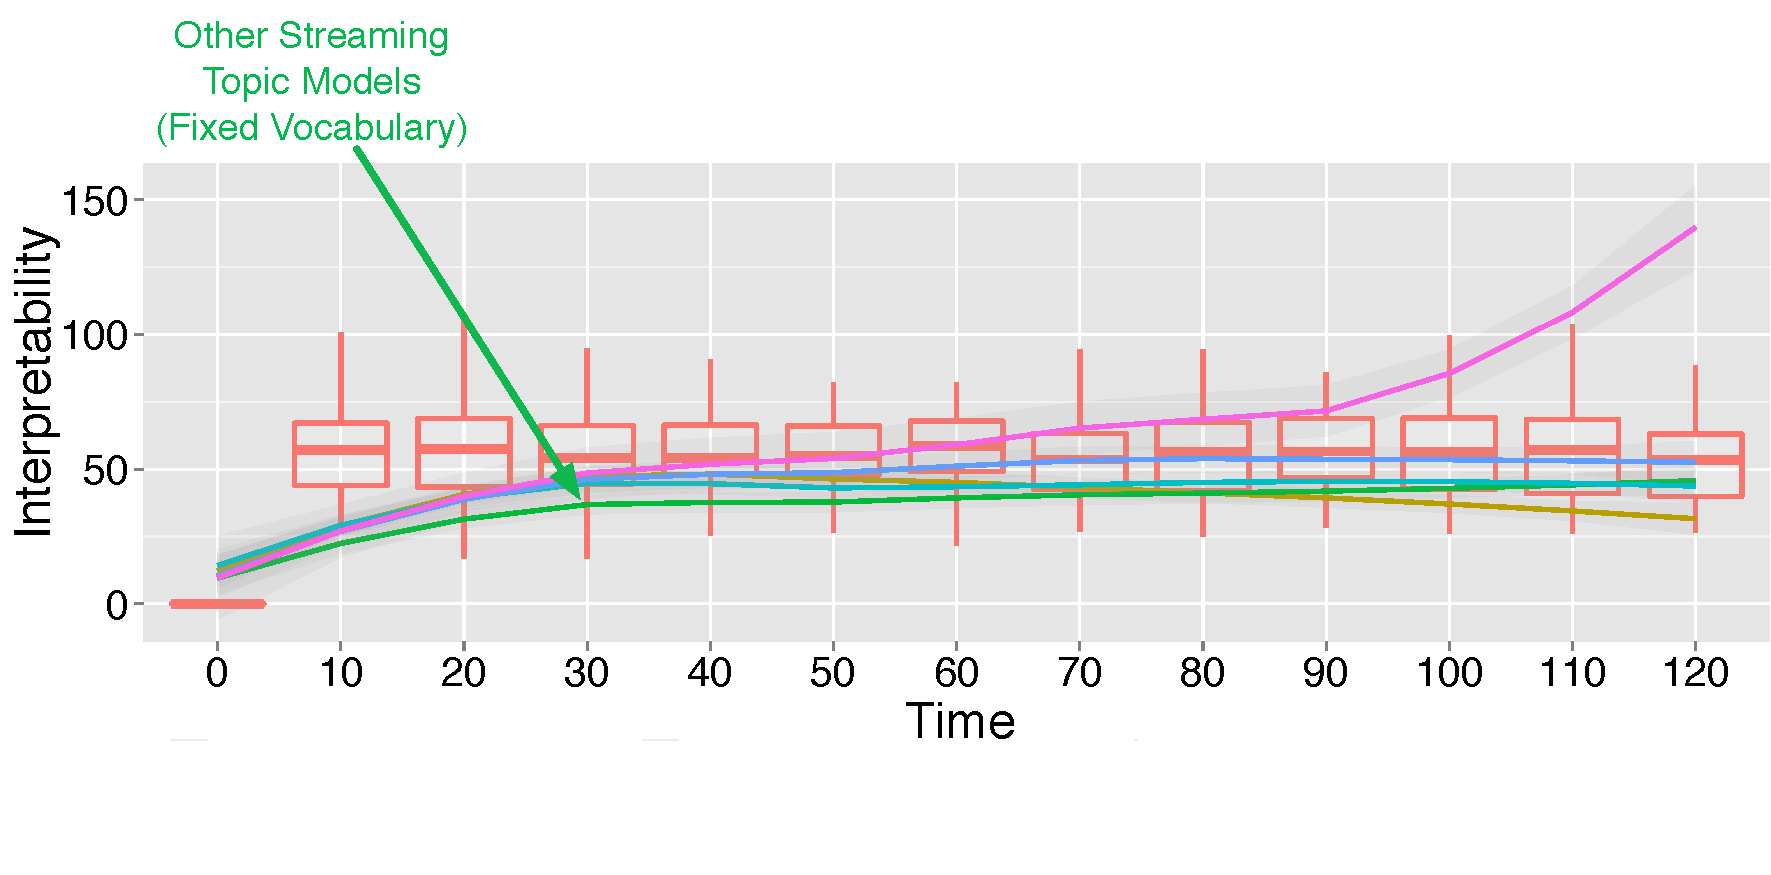
\includegraphics[width=1.0\linewidth]{infvoc/coherence_1}}
       \only<3>{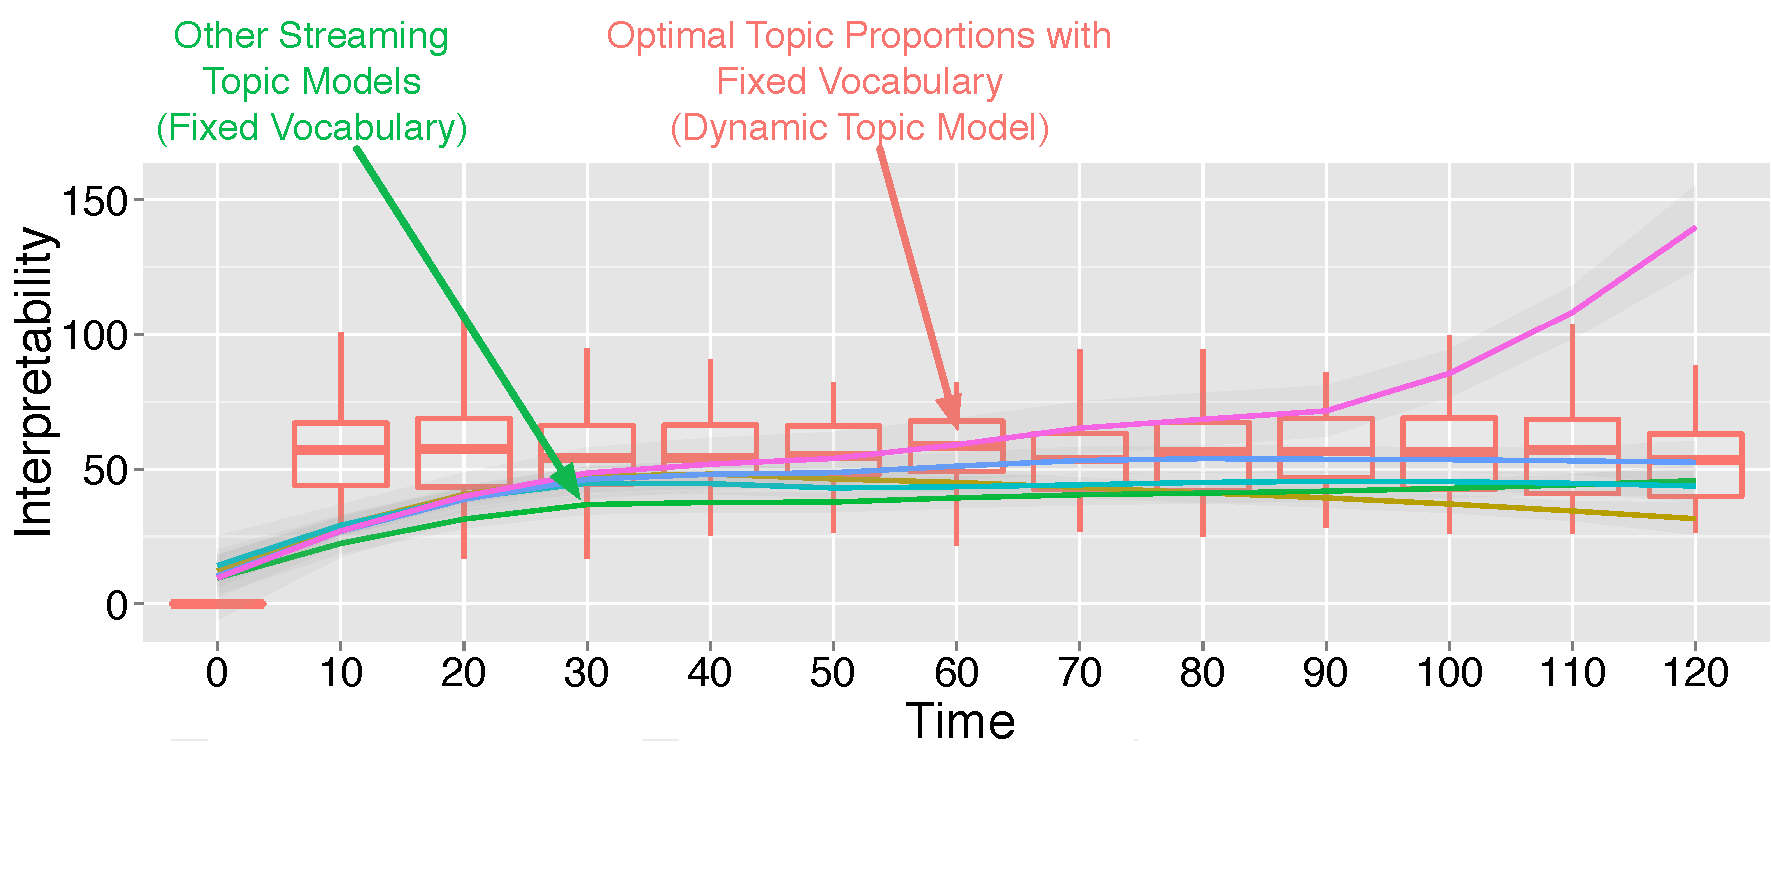
\includegraphics[width=1.0\linewidth]{infvoc/coherence_2}}
       \only<4>{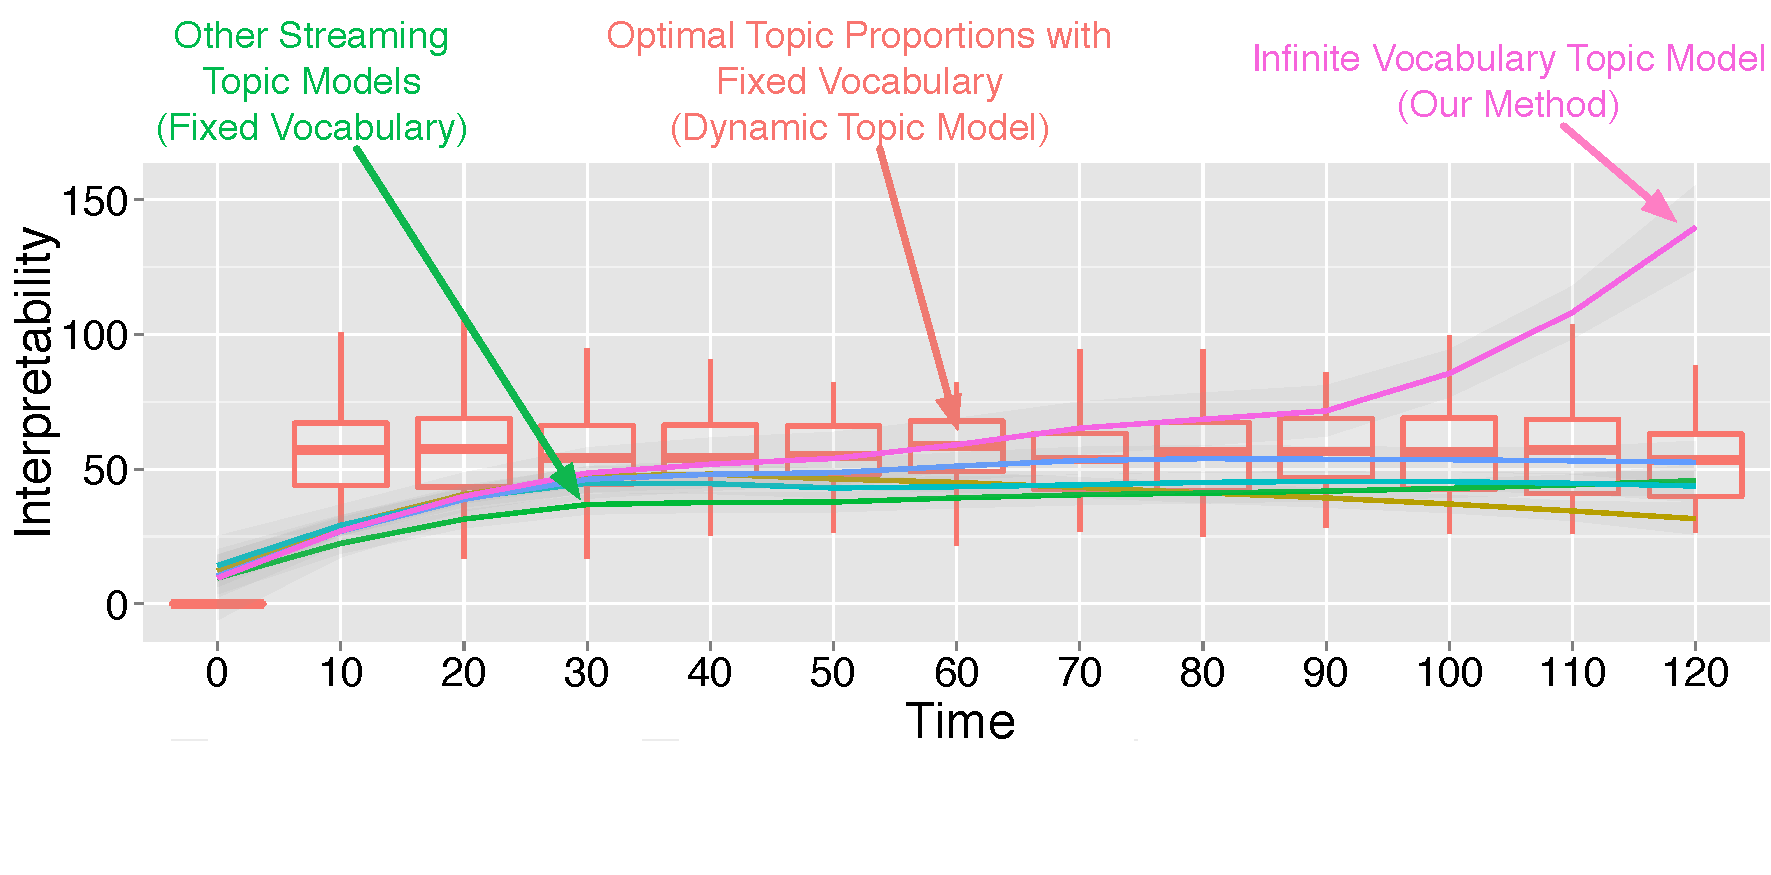
\includegraphics[width=1.0\linewidth]{infvoc/coherence_3}}

\begin{columns}
\column{.5\linewidth}
\begin{itemize}
  \item Finite topic models
  \item ``Dynamic'' topic models
\end{itemize}

\column{.5\linewidth}
\begin{itemize}
  \item Hashed vocabulary
  \item Other inference techniques
\end{itemize}
\end{columns}


\end{frame}
